\documentclass[a4paper, 12pt]{report}
\usepackage{cmap}
\usepackage[T2A]{fontenc}
\usepackage[utf8]{inputenc}
\usepackage[english,russian]{babel}
\usepackage{listings}
\usepackage{amsmath}
\usepackage{float}
\usepackage{csquotes}
\usepackage{graphicx}
\graphicspath{ {./images/} }
\usepackage{xcolor}
\definecolor{buzzlightyear}{HTML}{8757A5}
\definecolor{grass}{HTML}{738D06}
\definecolor{literal}{HTML}{F18A2B}
\definecolor{commentcolor}{HTML}{8E908B}

\lstdefinestyle{habrstyle}{
	backgroundcolor=\color{white},
	commentstyle=\color{commentcolor},
	keywordstyle=\bfseries\color{buzzlightyear},
	numberstyle=\tiny\color{commentcolor},
	stringstyle=\color{grass},
	basicstyle=\ttfamily\footnotesize,
	breakatwhitespace=false,         
    	breaklines=true,                 
   	captionpos=b,                    
    	keepspaces=true,                 
    	numbers=left,                    
    	numbersep=7pt,                  
    	showspaces=false,                
    	showstringspaces=false,
   	showtabs=false,                  
    	tabsize=3
}

\lstset{style=habrstyle}

\author{3530901/80201, Шелаев Н. Р.}
\title{Лабораторная работа № 10. Линейные стационарные системы.}
\date{\today}

\begin{document}
	\maketitle
	\tableofcontents
	\listoffigures
	\lstlistoflistings

	\chapter{Сигналы и системы}
	Линейная стационарная система - это система, которая линейна и неизменна во времени.
	\begin{lstlisting}[language=Python,caption=Строим импульс]
		from thinkdsp import Wave

		impulse = np.zeros(8)
		impulse[0] = 1
		wave = Wave(impulse, framerate = 8)
		impulse_spectrum = wave.make_spectrum(full=True)
	\end{lstlisting}
	\begin{lstlisting}[language=Python,caption=Исследуем полученный импульс]
		impulse = np.zeros(10000)
		impulse[0] = 1
		wave = Wave(impulse, framerate = 10000)
		wave.plot()
		wave.make_spectrum().plot()	
	\end{lstlisting}
	\begin{figure}[H]
		\centering
		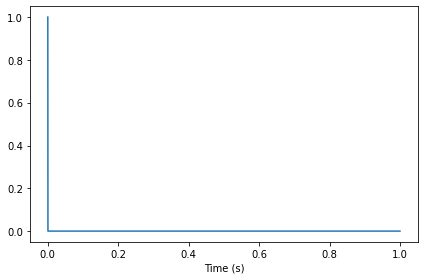
\includegraphics[width=0.75\textwidth]{imp1.png}
		\caption{Сигнал импульса}
		\label{fig:imp1}
	\end{figure}
	\begin{figure}[H]
		\centering
		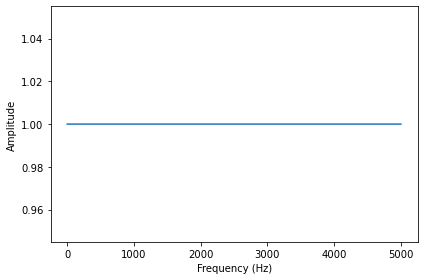
\includegraphics[width=0.75\textwidth]{imp2.png}
		\caption{Его спектр}
		\label{fig:imp2}
	\end{figure}

	\chapter{Окна и фильтры}
	Вычисление двухэлементного скользящего среднего.
	\begin{lstlisting}[language=Python,caption=Найдем двухэлементное скользящее среднее]
		window_array = np.array([0.5, 0.5, 0, 0, 0, 0, 0, 0,])
		window = Wave(window_array, framerate = 8)
		filtr = window.make_spectrum(full = True)
	\end{lstlisting}
	\begin{figure}[H]
		\centering
		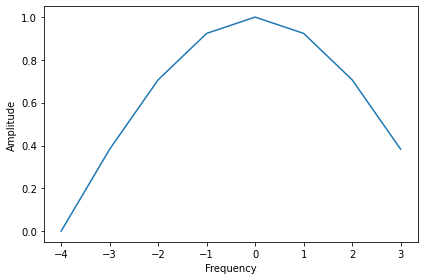
\includegraphics[width=0.75\textwidth]{sys1.png}
		\caption{ДПФ двухэлементного скользящего среднего}
		\label{fig:sys1}
	\end{figure}
	\begin{lstlisting}[language=Python,caption=Умножение передаточной функции на спектр импульса]
		product = impulse_spectrum * filtr
		filtered = product.make_wave()
	\end{lstlisting}
	\begin{figure}[H]
		\centering
		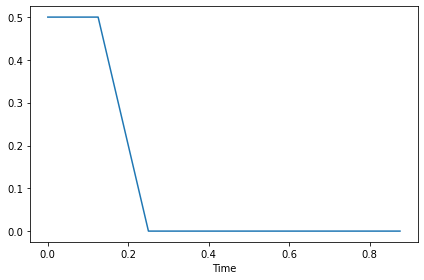
\includegraphics[width=0.75\textwidth]{sys2.png}
		\caption{Импульсная реакция}
		\label{fig:sys2}
	\end{figure}
	Запись импульсной характеристики достаточна для характеристики всей системы, потому что это \sloppy{\texttt{IDFT}} для передаточной функции.

	\chapter{Акустическая характеристика}
	Проведём исследование акустической характеристики некоторого пространства (например, комнаты).
	\begin{lstlisting}[language=Python,caption=Звук выстрела]
		from thinkdsp import read_wave

		response = read_wave('180960__kleeb__gunshot.wav')
		start = 0.12
		response = response.segment(start=start)
		response.shift(-start)
		response.normalize()
		response.plot()
	\end{lstlisting}
	\begin{figure}[H]
		\centering
		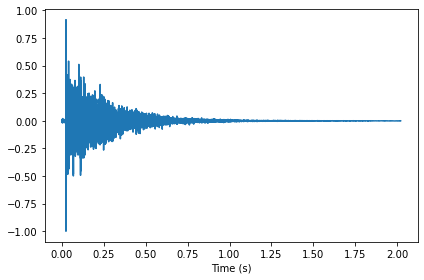
\includegraphics[width=0.75\textwidth]{shot1.png}
		\caption{Сегмент записи выстрела}
		\label{fig:shot1}
	\end{figure}
	\begin{lstlisting}[language=Python,caption=Строим спектр звука выстрела]
		transfer = response.make_spectrum()
		transfer.plot()
		decorate(xlabel = 'Frequency (Hz)', ylabel='Amplitude')
		
		transfer.plot()
		decorate(xlabel = 'Frequency (Hz)', ylabel='Amplitude', xscale = 'log', yscale = 'log')
	\end{lstlisting}
	\begin{figure}[H]
		\centering
		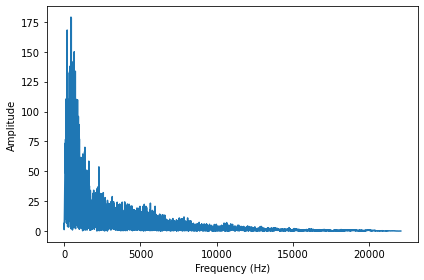
\includegraphics[width=0.75\textwidth]{shot2.png}
		\caption{Спектр звука выстрела}
		\label{fig:shot2}
	\end{figure}
	\begin{figure}[H]
		\centering
		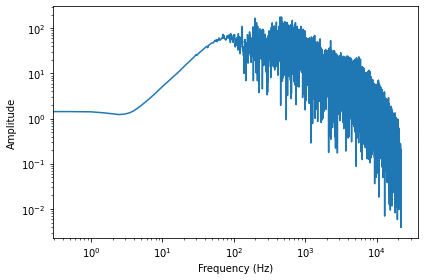
\includegraphics[width=0.75\textwidth]{shot3.png}
		\caption{Спектр в логарифмическом масштабе}
		\label{fig:shot3}
	\end{figure}
	Спектр соответствует отклику комнаты. Каждая частота в спектре представлена комплексным числом в виде амплитуды и фазы. Этот спектр называется \sloppy{Передаточной функцией}.
	\begin{lstlisting}[language=Python,caption=Звук скрипки]
		violin = read_wave('92002__jcveliz__violin-origional.wav')
		start = 0.11
		violin = violin.segment(start = start)
		violin.shift(-start)
		violin.truncate(len(response))
		violin.normalize()
		violin.plot()
		spectrum = violin.make_spectrum()
		spectrum.plot()
	\end{lstlisting}
	\begin{figure}[H]
		\centering
		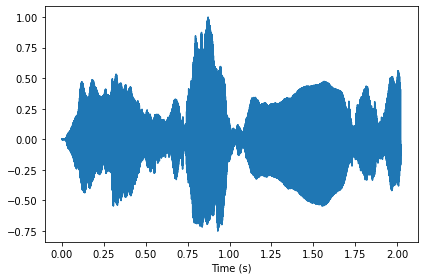
\includegraphics[width=0.75\textwidth]{shot4.png}
		\caption{Сегмент звука скрипки}
		\label{fig:shot4}
	\end{figure}
	\begin{figure}[H]
		\centering
		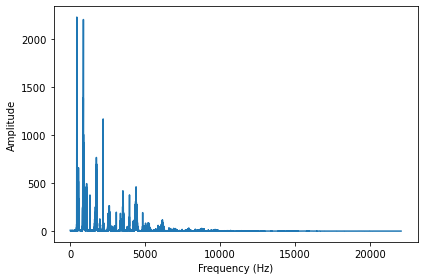
\includegraphics[width=0.75\textwidth]{shot5.png}
		\caption{Спектр этого звука}
		\label{fig:shot5}
	\end{figure}
	\begin{lstlisting}[language=Python,caption=Вычисление выходного сигнала]
		output = (spectrum * transfer).make_wave()
		violin.plot()
		output.plot()
		spectrum = output.make_spectrum()
		spectrum.plot()
	\end{lstlisting}
	\begin{figure}[H]
		\centering
		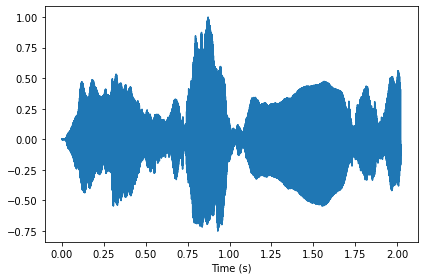
\includegraphics[width=0.75\textwidth]{shot6.png}
		\caption{Оригинальный звук}
		\label{fig:shot6}
	\end{figure}
	\begin{figure}[H]
		\centering
		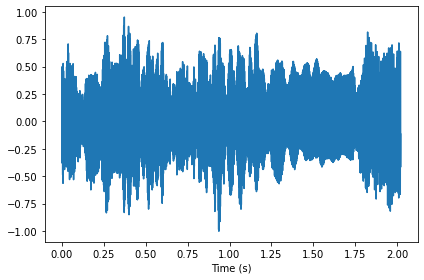
\includegraphics[width=0.75\textwidth]{shot7.png}
		\caption{Преобразованная запись}
		\label{fig:shot7}
	\end{figure}
	\begin{figure}[H]
		\centering
		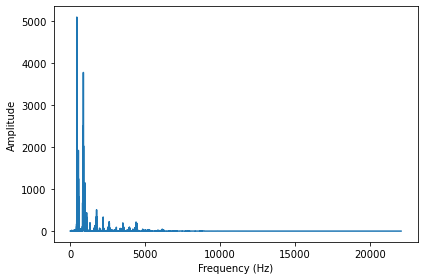
\includegraphics[width=0.75\textwidth]{shot8.png}
		\caption{Спектр преобразованного звука}
		\label{fig:shot8}
	\end{figure}
	Разница между этими двумя звуками хорошо различима на слух.

	\chapter{Системы и свертка}
	Выход системы - свертка входа и отклика системы.
	\begin{lstlisting}[language=Python,caption=Создадим звук двух последовательных выстрелов]
		def shifted_scaled(wave, shift, factor):
			res = wave.copy()
			res.shift(shift)
			res.scale(factor)
			return res

		response2 = response + shifted_scaled(response, 1, 0.5)
		response2.plot()
	\end{lstlisting}
	\begin{figure}[H]
		\centering
		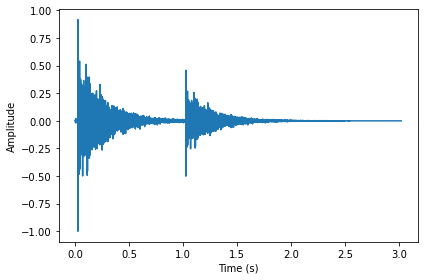
\includegraphics[width=0.75\textwidth]{shot9.png}
		\caption{Два выстрела}
		\label{fig:shot9}
	\end{figure}
	\begin{lstlisting}[language=Python,caption=Очень много последовательных выстрелов]
		dt = 1 / 441
		total = 0
		for k in range(220):
			total += shifted_scaled(response, k * dt, 1.0)
		
		total.normalize()
		total.plot()
	\end{lstlisting}
	\begin{figure}[H]
		\centering
		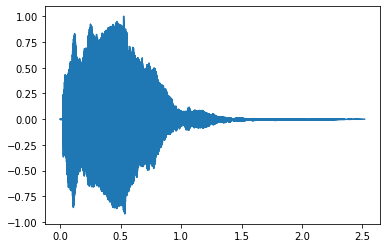
\includegraphics[width=0.75\textwidth]{shot10.png}
		\caption{Теперь это уже не похоже на звук выстрела}
		\label{fig:shot10}
	\end{figure}
	\begin{lstlisting}[language=Python,caption=Произвольный входной сигнал]
		from thinkdsp import SawtoothSignal

		signal = SawtoothSignal(freq = 441)
		wave = signal.make_wave(duration=0.2, framerate=response.framerate)
		wave.plot()
	\end{lstlisting}
	\begin{figure}[H]
		\centering
		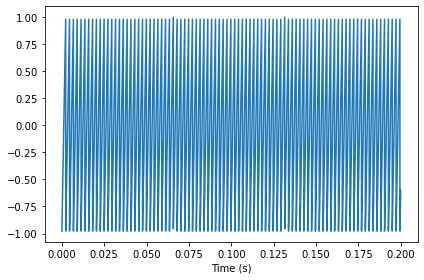
\includegraphics[width=0.75\textwidth]{shot11.png}
		\caption{Произвольный сигнал}
		\label{fig:shot11}
	\end{figure}
	\begin{lstlisting}[language=Python,caption=Генерация сдвинутых версий импульсной характеристики]
		total = 0
		for t, y in zip(wave.ts, wave.ys):
			total += shifted_scaled(response, t, y)
		
		total.normalize()
		total.plot()
	\end{lstlisting}
	\begin{figure}[H]
		\centering
		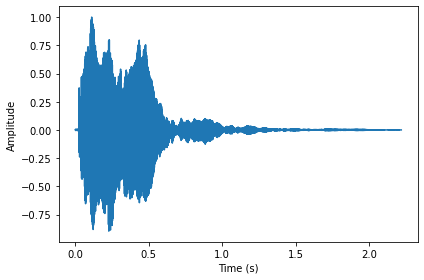
\includegraphics[width=0.75\textwidth]{shot12.png}
		\caption{Чем-то похоже на звук двух последовательных выстрелов}
		\label{fig:shot12}
	\end{figure}
	\begin{lstlisting}[language=Python,caption=Используем метод свертки]
		high = 5000
		wave.make_spectrum().plot(high = high, color = '0.7')
		segment = total.segment(duration = 0.2)
		segment.make_spectrum().plot(high = high)
		convolved2 = violin.convolve(response)
		convolved2.plot()
	\end{lstlisting}
	\begin{figure}[H]
		\centering
		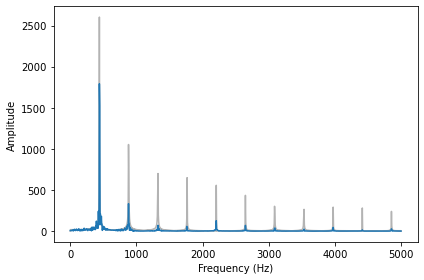
\includegraphics[width=0.75\textwidth]{shot13.png}
		\caption{Сравнение спектра до и после свертки}
		\label{fig:shot13}
	\end{figure}
	\begin{figure}[H]
		\centering
		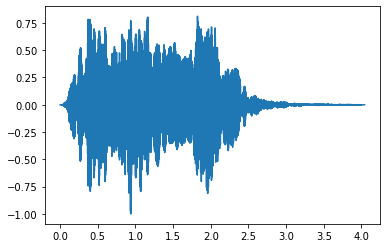
\includegraphics[width=0.75\textwidth]{shot14.png}
		\caption{Результат свертки}
		\label{fig:shot14}
	\end{figure}
	
	\chapter{Упражнения}
	\section{Задание 1}
	Устранение лишней ноты в начале фрагмента сигнала через дополнение нулями.
	\begin{lstlisting}[language=Python,caption=Сначала возьмём звук выстрела]
		response = read_wave('180960__kleeb__gunshot.wav')
		start = 0.12
		response = response.segment(start=start)
		response.shift(-start)
		response.truncate(2 ** 16)
		response.zero_pad(2 ** 17)
		response.normalize()
		response.plot()
		transfer = response.make_spectrum()
		transfer.plot()
	\end{lstlisting}
	\begin{figure}[H]
		\centering
		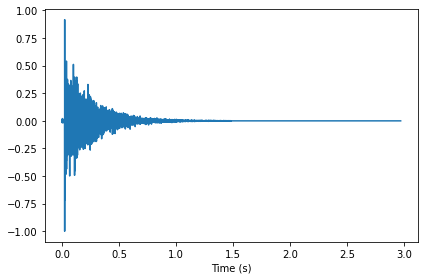
\includegraphics[width=0.75\textwidth]{task1.png}
		\caption{Исправленный звук выстрела}
		\label{fig:task1}
	\end{figure}
	\begin{figure}[H]
		\centering
		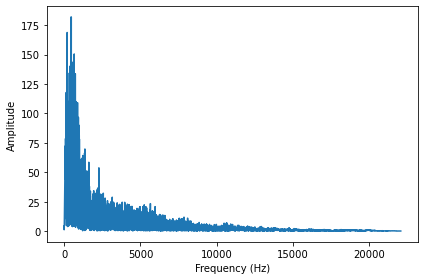
\includegraphics[width=0.75\textwidth]{task2.png}
		\caption{И его спектр}
		\label{fig:task2}
	\end{figure}
	\begin{lstlisting}[language=Python,caption=Теперь попробуем с сигналом скрипки]
		violin = read_wave('92002__jcveliz__violin-origional.wav')
		start = 0.11
		violin = violin.segment(start = start)
		violin.shift(-start)
		violin.truncate(2 ** 16)
		violin.zero_pad(2 ** 17)
		violin.normalize()
	\end{lstlisting}
	\begin{figure}[H]
		\centering
		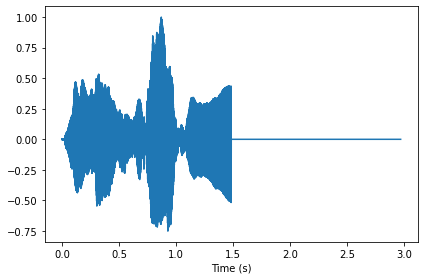
\includegraphics[width=0.75\textwidth]{task3.png}
		\caption{Исправленный сигнал скрипки}
		\label{fig:task3}
	\end{figure}
	\begin{lstlisting}[language=Python,caption=Перемножаем спектры]
		spectrum = violin.make_spectrum()
		output = (spectrum * transfer).make_wave()
		output.normalize()
		output.plot()
	\end{lstlisting}
	\begin{figure}[H]
		\centering
		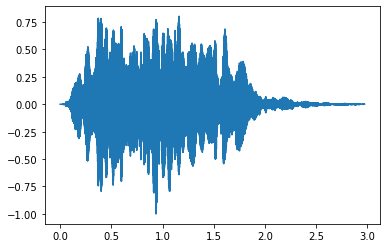
\includegraphics[width=1.0\textwidth]{task4.png}
		\caption{Умножение на передаточную функцию}
		\label{fig:task4}
	\end{figure}
	\begin{lstlisting}[language=Python,caption=Убираем нули в конце сигналов]
		response.truncate(2 ** 16)
		response.plot()
		violin.truncate(2 ** 16)
		violin.plot()
	\end{lstlisting}
	\begin{figure}[H]
		\centering
		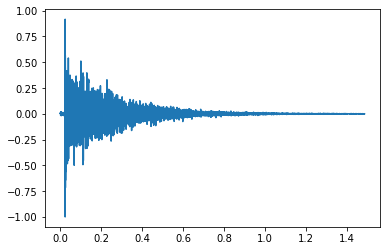
\includegraphics[width=0.75\textwidth]{task5.png}
		\caption{Звук выстрела без нулей}
		\label{fig:task5}
	\end{figure}
	\begin{figure}[H]
		\centering
		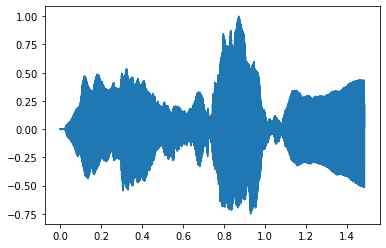
\includegraphics[width=0.75\textwidth]{task6.png}
		\caption{Сигнал скрипки тоже без нулей}
		\label{fig:task6}
	\end{figure}
	\begin{lstlisting}[language=Python,caption=Свертка сигнала скрипки]
		output2 = violin.convolve(response)
		output2.plot()
	\end{lstlisting}
	\begin{figure}[H]
		\centering
		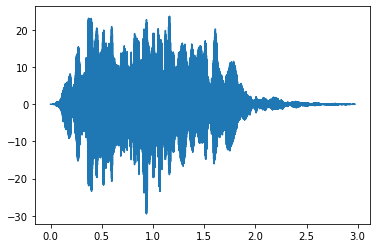
\includegraphics[width=0.75\textwidth]{task7.png}
		\caption{Результат свертки}
		\label{fig:task7}
	\end{figure}
	Результаты похожи по графикам и звуку, но \sloppy{\texttt{len(output2)}} = \sloppy{\texttt{len(output)}} - 1. 
	\begin{lstlisting}[language=Python,caption=Свертка сигнала скрипки с помощью FFT]
		import scipy.signal
		from thinkdsp import Wave

		ys = scipy.signal.fftconvolve(violin.ys, response.ys)
		output3 = Wave(ys, framerate = violin.framerate)
		output3.plot()
	\end{lstlisting}
	\begin{figure}[H]
		\centering
		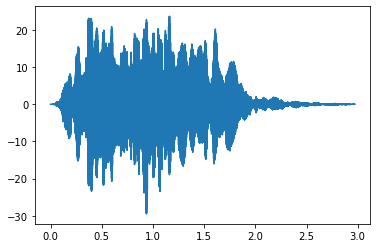
\includegraphics[width=0.75\textwidth]{task8.png}
		\caption{Результат свертки с помощью другой функции}
		\label{fig:task8}
	\end{figure}
	Разница между результатами работы первой и второй функций близка к 0, но вторая функция работает гораздо быстрее.

	\section{Задание 2}
	Моделирование звучания записи в том пространстве, где была измерена импульсная характеристика.
	\begin{lstlisting}[language=Python,caption=Сначала попробуем какой-то звук]
		response = read_wave('stalbans_a_mono.wav')
		response = response.segment(duration = 5)
		response.shift(-0)
		response.normalize()
		response.plot()
		transfer = response.make_spectrum()
		transfer.plot()
		decorate(xlabel = 'Frequency (Hz)', ylabel='Amplitude')

		transfer.plot()
		decorate(xlabel = 'Frequency (Hz)', ylabel='Amplitude', xscale = 'log', yscale = 'log')
	\end{lstlisting}
	\begin{figure}[H]
		\centering
		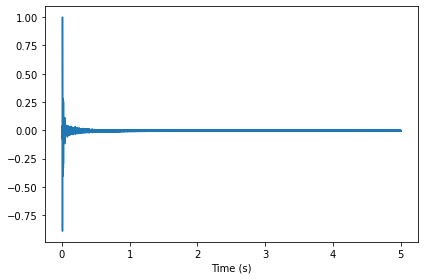
\includegraphics[width=0.75\textwidth]{task9.png}
		\caption{Сигнал импульса}
		\label{fig:task9}
	\end{figure}
	\begin{figure}[H]
		\centering
		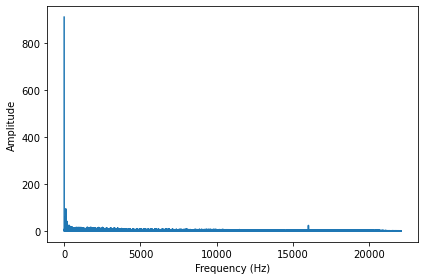
\includegraphics[width=0.75\textwidth]{task10.png}
		\caption{Спектр импульса}
		\label{fig:task10}
	\end{figure}
	\begin{figure}[H]
		\centering
		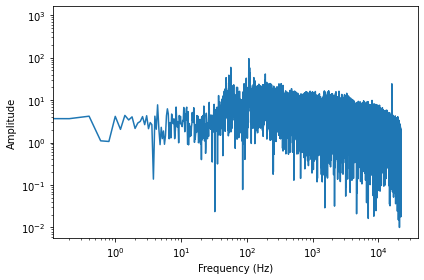
\includegraphics[width=0.75\textwidth]{task11.png}
		\caption{Спектр импульса в логарифмическом масштабе}
		\label{fig:task11}
	\end{figure}
	Теперь мы можем смоделировать, как звучала бы запись, если бы она воспроизводилась в той же комнате и записывалась таким же образом.
	\begin{lstlisting}[language=Python,caption=Запись игры на трубе]
		wave = read_wave('170255__dublie__trumpet.wav')
		start = 0.0
		wave = wave.segment(start = start)
		wave.shift(-start)
		wave.truncate(len(response))
		wave.normalize()
		wave.plot()
	\end{lstlisting}
	\begin{figure}[H]
		\centering
		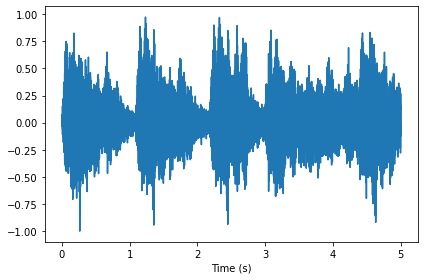
\includegraphics[width=0.75\textwidth]{task12.png}
		\caption{Сигнал записи игры на трубе}
		\label{fig:task12}
	\end{figure}
	\begin{lstlisting}[language=Python,caption=Перемножаем спектры для этого сигнала]
		spectrum = wave.make_spectrum()
		output = (spectrum * transfer).make_wave()
		output.normalize()
		wave.plot()
		output.plot()
	\end{lstlisting}
	\begin{figure}[H]
		\centering
		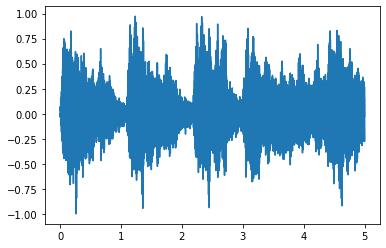
\includegraphics[width=0.75\textwidth]{task13.png}
		\caption{Оригинальная запись}
		\label{fig:task13}
	\end{figure}
	\begin{figure}[H]
		\centering
		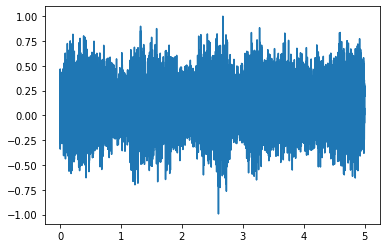
\includegraphics[width=0.75\textwidth]{task14.png}
		\caption{Изменённая запись сигнала}
		\label{fig:task14}
	\end{figure}
	Теперь кажется, что запись игры на трубе делали там же, где записывали импульс. Аналогичное решение можно получить, применив встроенную функцию свертки \sloppy{\texttt{fftconvolve}}.

	\chapter{Вывод}
	В данной работе мы познакомились с линейными стационарными системами и акустическими характеристиками пространства. Также использовали различные методы для получения выхода системы по входному сигналу и отклику этой системы.
\end{document}